
\section{Experimental Setup}
% Need to be approximately 7 pages:
% 1 page for general words
% 2 pages for neutrino beam, near detector and far detector

The Long Beamline Neutrino Facility is the facility being internationally designed for the future Deep Underground Neutrino Experiment (DUNE) which has wide physics program for variety of precision measurements and searches beyond the Standard Model. The general scheme of the facility is shown on figure \ref{fig:LBNF_overallScheme}. This section gives more details on neutrino beam production and the detector descriptions. The information if taken mostly from the LBNF website[REFERENCE] and the Conceptual Design Report which is currenly under development but drafts are partially available [REFERENCE].
The first collaboration meeting took place on April 16th-18th of 2015 in Fermilab [REFERENCE]. There were about 200 participants out of total of 750 members. The statuses and prospectives of the Near Detector, Far Detector, Neutrino beam, software infrastructure and other related technical topics were discussed. Most information written in this section is taken from the presentations of this collaboration meeting, the CDR drafts and the main pages of the LFNF website [REFERENCE].

\begin{figure}
\caption{Fermilab Accelerator Complex}
\label{fig:LBNF_FermilabAccComplex}
\centering
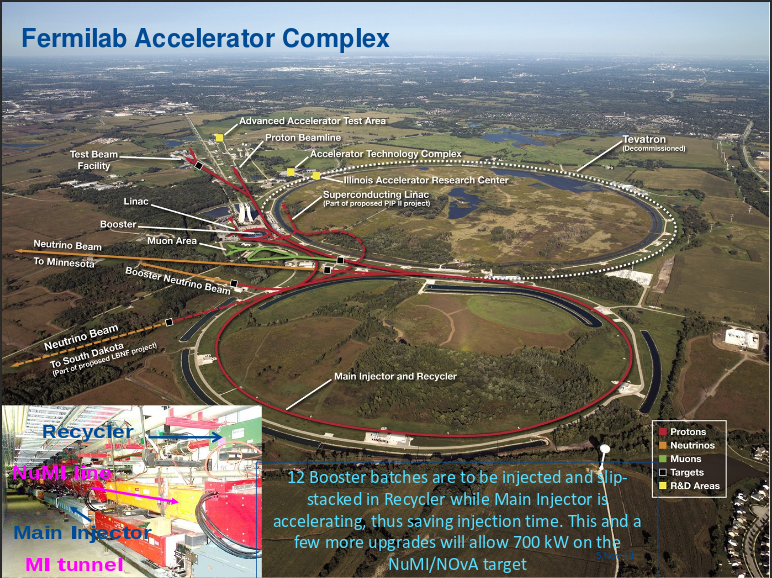
\includegraphics[width=0.95\textwidth, keepaspectratio=true]{figs/FermilabAccelerator.png}
\\The Fermilab Accelerator Complex as it is described in the presentation "The LBNF Beamline and PIP-II" by Vaia Papadimitriou at the fisrt LBNF Collaboration meeting [REFERENCE].   
\end{figure}

\begin{figure}
\caption{Long Baseline Neutrino Facility}
\label{fig:LBNF_overallScheme}
\centering
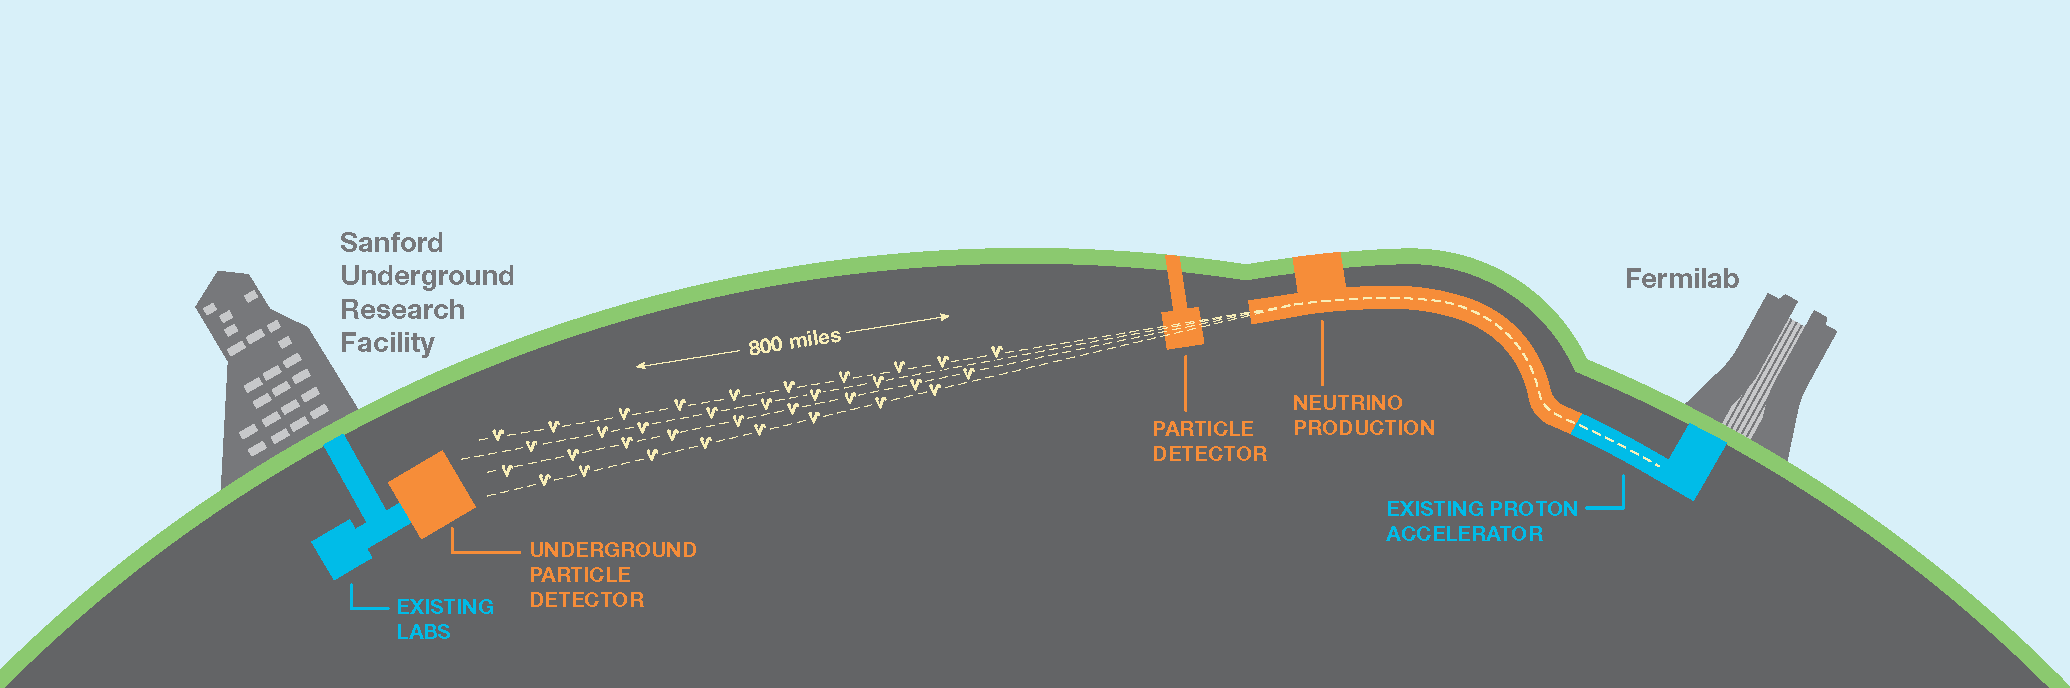
\includegraphics[width=0.95\textwidth, keepaspectratio=true]{figs/LBNF_overallScheme.png}
\\The neutrino flux will be produced using existing proton accelerator in Fermilab. Then neutrinos will be registered by near detector, travel 800 miles through the Earth mantle to the Sanford Underground Research Facility in South Dakota and be registed by far detector. \cite{ref_LBNFweb}   
\end{figure}

Scheme of the Fermilab accelerator complex is shown at the (fig. \ref{fig:LBNF_FermilabAccComplex} ) and the overall scheme of the 
Long Baseline Neutrino Facility (LBNF) is shown at the (fig. \ref{fig:LBNF_overallScheme} ). The protons from the accelerator  will induce the neutrino beam which will be travel trough the Earth in direction of the Deep Underground Neutrino Experiment (DUNE) detector in South Dakota. It is common for the long baseline neutrino oscillations experiments to have a near detector (several hundred meters from the neutrino production) and far detector (hundreds of kilometers away). Comparing measurements of neutrino flux characteristics at two points allows to extract parameters of neutrino oscillations physics.

General requirements for the experiment are listed in [REFERENCE].
\begin{itemize}
  \item neutrino beam of high intensity which would be able to produce large amount of neutrinos to be registered at the far site
  \item the detector to register neutrinos and measure the beamline characteristics at the near site
  \item the liquid argon time-projection chamber for the far site detector (LArTPC)
\end{itemize}

\subsection{Neutrino Beam}

\begin{figure}
\caption{Neutrino beam of the LBNF}
\label{fig:LBNF_nuBeam}
\centering
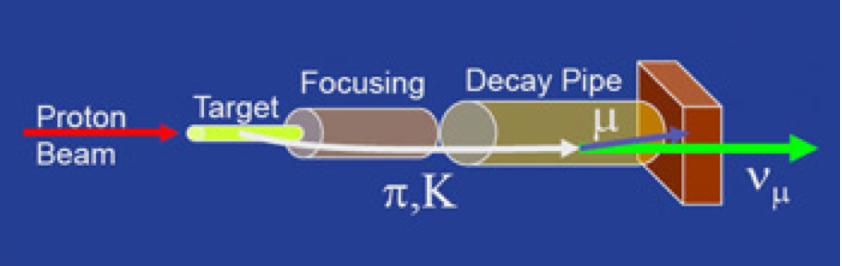
\includegraphics[width=0.45\textwidth, keepaspectratio=true]{figs/LBNF_nuBeam.png}
\\The neutrino beam production at Long Beamline Neutrino Facility. \cite{ref_LBNFweb}   
\end{figure}


\begin{figure}
\caption{Charged pion and kaon productions}
\label{fig:pionAndKaonProductions}
\centering
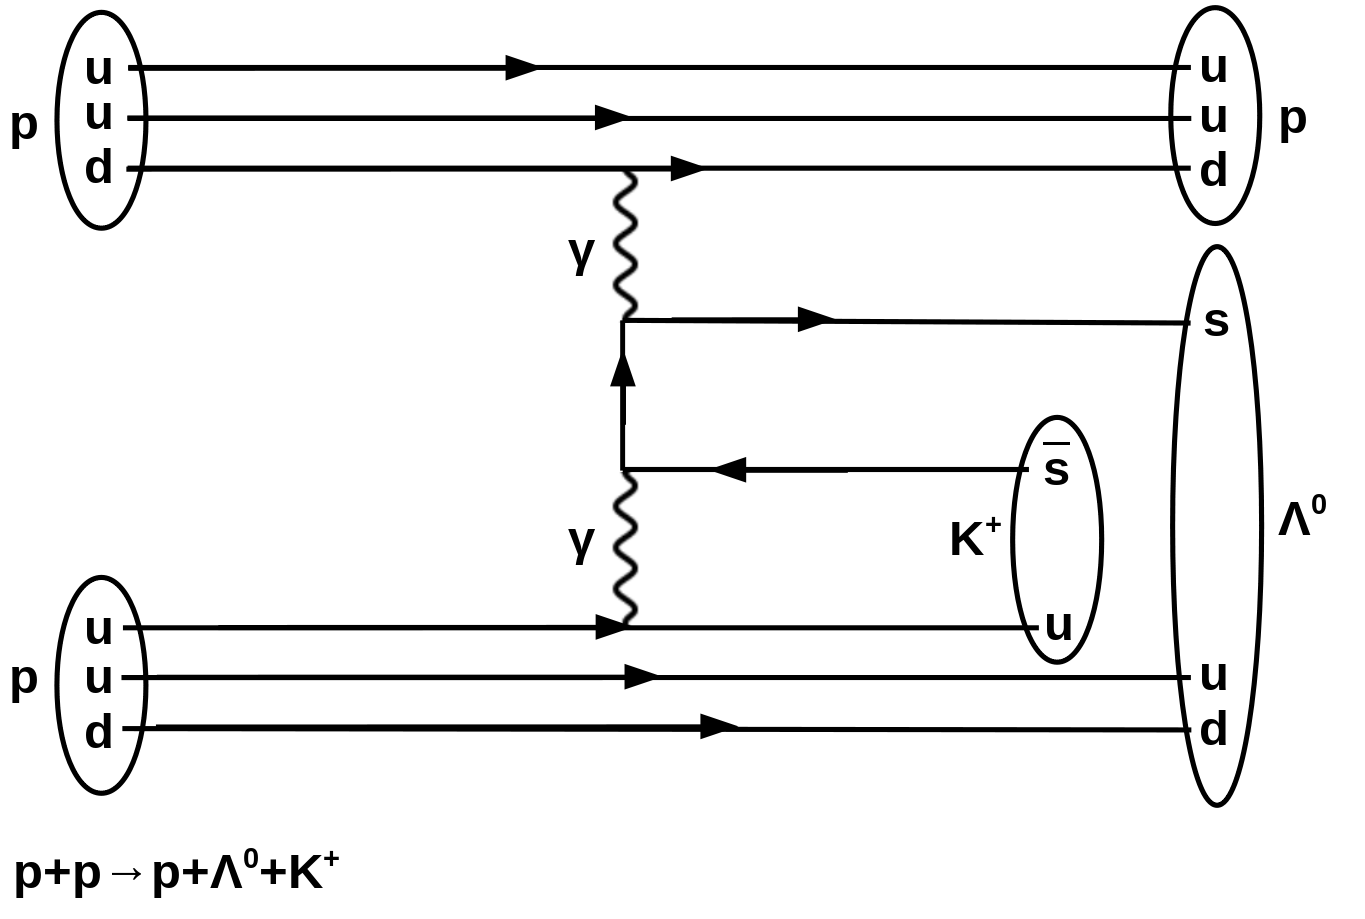
\includegraphics[width=0.48\textwidth, keepaspectratio=true]{figs/ppKaonProduction.png}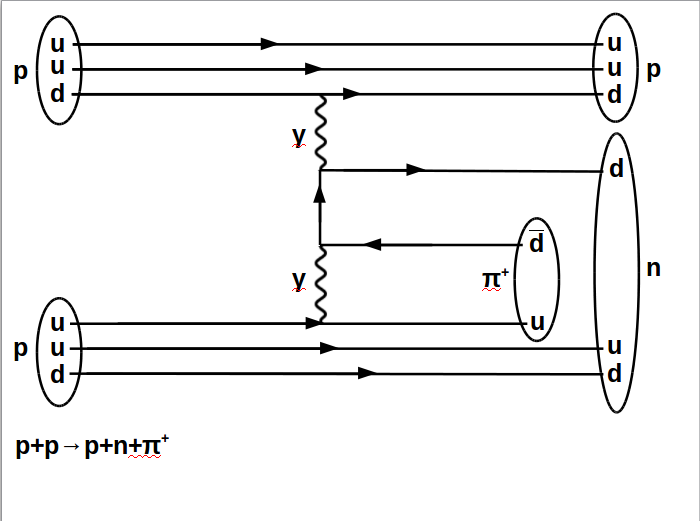
\includegraphics[width=0.48\textwidth, keepaspectratio=true]{figs/ppPionProduction.png}
\\Exmples of Feynmann diagrams of chagred kaons and pions production in proton-proton scattering.    
\end{figure}


It's going to use the highest intensity neutrino beam ever created. The proton accelerator in Fermilab which was already used in other experiments in Fermilab before will produce the beam of protons. Then protons will hit a target and create kaons and pions through the same reactions as take place in atmosphere when the cosmic protons hit molecules of air.  Pions can be created in the reactions $p+p \rightarrow p+n+\pi^+$, $p+p \rightarrow p+\Delta^{++}+\pi^-$, $p+n \rightarrow p+p+\pi^-$, $p+n \rightarrow n+n+\pi^+$, $p+n \rightarrow p+\Delta^{-}+\pi^+$ etc which go electromagnetically though photon. In more general words, one quark from the accelerator beam proton scatters on the other quark from the proton or neutron of the target substance. They exchange photon which produces quark-antiquark pair. At this moment, the system has seven quarks and one antiquark. The antiquark pairs up with one of the quarks participating in the reaction and the remaining six quarks make two baryons.  The charged pions have formulas $\pi^+ = u\bar{d}$ and $\pi^- = \bar{u}d$ and can be produced with the reactions which only include first generation quarks. The formulas of charged kaons are $K^+ = u\bar{s}$, $K^- = \bar{u}s$. Thus, to produce kaons, the photon has to produce $s\bar{s}$ pair. 

\begin{figure}
\caption{Charged pion and kaon decays}
\label{fig:pionAndKaonDecays}
\centering
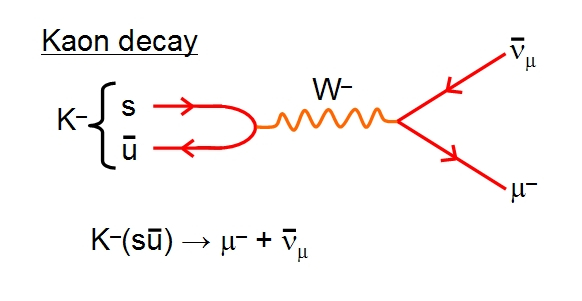
\includegraphics[width=0.45\textwidth, keepaspectratio=true]{figs/kaonDecay.jpg}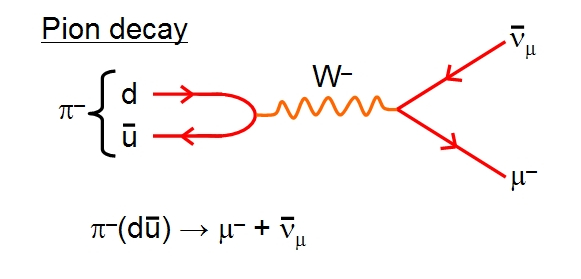
\includegraphics[width=0.45\textwidth, keepaspectratio=true]{figs/pionDecay.jpg}
\\Feynmann diagrams of charged pion and kaon decays to muon and muon antineutrino weakly through W-boson. Picture taken from \cite{ref_fig_pionandKaonDecays}.   
\end{figure}

After the mesons are created, they go through the focusing camera and decay into the decay pipe (the length of the decay pipe is about 200 meters) as $\pi^+ \rightarrow \mu^+\nu_\mu$, $\pi^- \rightarrow \mu^-\bar{\nu_\mu}$, $K^+ \rightarrow \mu^+\nu_\mu$, $K^- \rightarrow \mu^-\bar{\nu_\mu}$. The branching ratios of charged pions and kaons to decay into $\mu^+\nu_\mu$($\mu^-\bar{\nu_\mu}$) are $(>99.9)\%$ and $(63.55\pm0.011)\%$ respectively therefore most neutrinos produced into the decay pipe will be muon neutrinos. (While the neutral kaons can also be produced in the target and later decay in pions which could further decay and produce muon neutrinos, but the focusing is being done with the certain configuration of the magnetic field and thus only charged particles can be focused. Neutral pions, $\pi^0$s, are very likely to be produced as well but they decay as $\pi^0 \rightarrow \gamma\gamma$ and thus can't contribute to the neutrino production.)

After being produced in the rections described above, the neutrinos will be detected in the close detector in the Fermilab. Then the neutrinos will travel 800 miles underground and will be detected by Sanford Underground Research Facility in South Dakota.\\*  

Beam requirements listed in the "Beam Requirements and Beam Optimization talk" during the first LBNF collaboaration meeting include:
\begin{itemize}
  \item the beam must have high intensity, be wide-band
  \item must be able to produce muon neutrinos or antineutrinos by experimenter's choice
  \item fraction of the opposite sign neutrinos must be small
  \item the energy range of the first oscillation node (1-5 GeV) must be fully covered
  \item the second oscillation node, $\sim{0.8}$ GeV must be achievable too
  \item must work at $>\sim{2} $ MW at 60-120 GeV/c
  \item the option to tuned the lower primary proton momenta down to 60 GeV/c must present
  \item the systematic error to the parameters of the neutrino flux must be reduced
  \item the parameters of the neutrino flux must be stable
\end{itemize}

\subsection{Near Detector}


A near detector is an important part of any long baseline neutrino oscillation experiment. It measures the primary neutrino beam flux as it is produced by the beam production system. Chapter 6 of the draft LBNF Conceptual Design Report [REFERENCE] lists the following precision measurements to be performed by the Near Detector: 
\begin{itemize}
  \item absolute flux measurement
  \item relative neutrino and antineutrino flux measurements
  \item flavor content of the neutrino source
  \item determination of the $E_\nu$-scale of neutrinos versus antineutrinos
  \item event-by-event measurements of NC interactions
  \item measurement of $\pi^0$, $\pi^\pm$, $K^\pm$, p, $K^0_S$ and $\Lambda$ in the NC and CC
%  \item "quasi-elastic and resonance measurements"
  \item nucleon structure, parton distribution functions and QCD studies
  \item neutrino-argon interactions and nuclear effects
  \item precision measurements of electroweak physics
%  \item isospin physics and the Adler sum rule
%  \item measurement of the nuclean strangeness content
\end{itemize}

More specifically, the list of the physics measurements related to the neutrino oscillations to be performed by the Near Detector includes:
\begin{itemize}
  \item fluxes of $\nu_\mu$, $\bar{\nu_\mu}$, $\nu_e$ and $\bar{\nu_e}$. To distinguish between flavors, the measurement should rely on charged current interaction (fig. \ref{fig:MuonAndNeutronDecays}, middle and right) and measure the products of these interactions $\mu^-$, $\mu^+$, $e^-$, and $e^+$. (While the production has the highest probability to produce muon neutrinos, the production of certain number electron neutrinos is also possible, for example, from charged kaon decays)
  \item $\nu_e$-$\bar{\nu_e}$ assymetries for which will help with CP-violating phase measurement. For that, it's important not only distinguish between $\mu^\pm$ and $e^\pm$ but also between $e^-$ and $e^+$.
  \item the absolute $\nu_\mu$ and $\bar{\nu_\mu}$ fluxes need to be measured with $\simeq{3\%}$ precision in the neutrino energy range 0.5-8 GeV
  \item cross section of NC versus CC processes as a function of hadronic energy. NC is one of major backrounds which contribute to neutrino oscillation measurement
  \item yields of $\pi_0$ and photons. These particles are the most significant background to $\nu_e$ and $\bar{\nu_e}$ contamination
  \item fractions of the $\pi^\pm$ into the CC and the NC hadronic jets.    
\end{itemize} 

%\begin{SCfigure}
%side caption
%\caption{Scheme of the Near Detector. The detector will consist of central Straw-Tube Tracker (STT) modules, electromagnetic calorimeter (ECAL), magnet coils of 0.4T and muon identification system consisting of Resistive Plate Chamber (RPC) modules. The neutrinos would come from the bottom left corner of the picture, to the End RPCs. Source of figure: [REFERENCE]}
%\label{fig:nearDetector}
%\centering
%\includegraphics[width=0.50\textwidth, keepaspectratio=true]{figs/%nearDetector.png}
%\end{SCfigure}

\begin{figure}
\caption{Scheme of the Near Detector (left) and related complex (right).}
\label{fig:nearDetector}
\centering
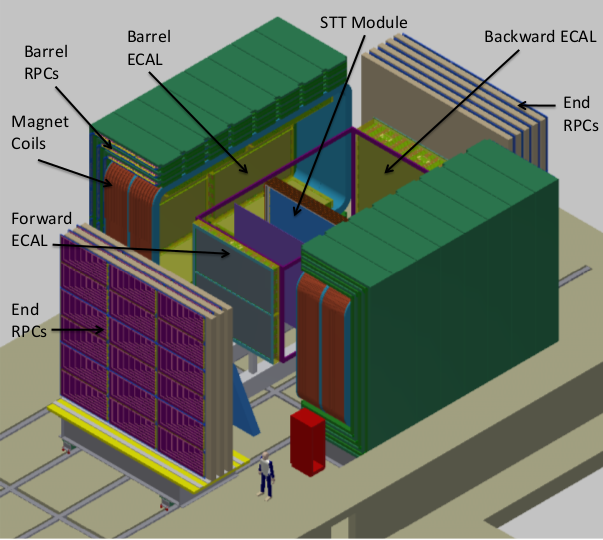
\includegraphics[width=0.63\textwidth, keepaspectratio=true]{figs/nearDetector.png}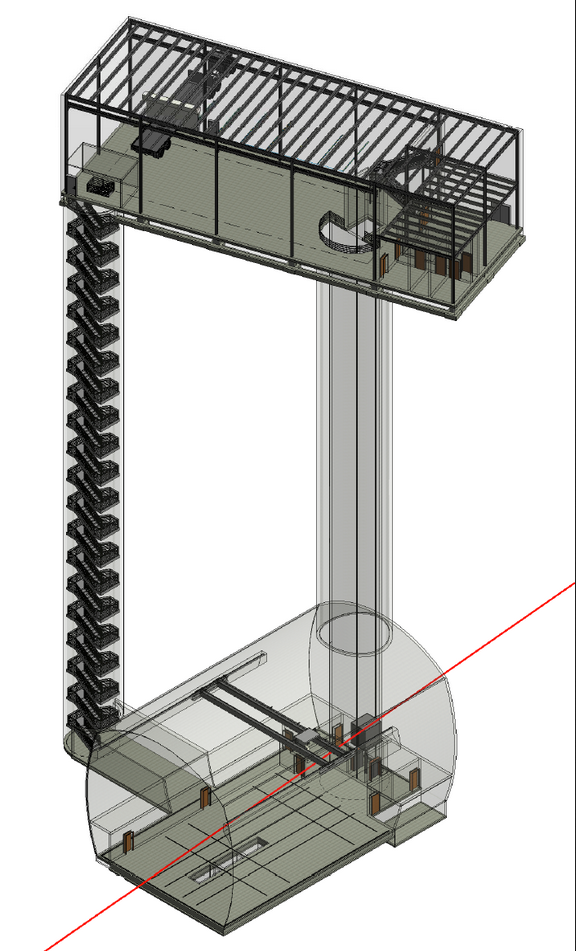
\includegraphics[width=0.35\textwidth, keepaspectratio=true]{figs/nearDetector_project.png}
\end{figure}

The scheme of the near detector is shown at the fig. \ref{fig:nearDetector}. The detector will consist of central Straw-Tube Tracker (STT) modules, electromagnetic calorimeter (ECAL), magnet coils of 0.4T and muon identification system consisting of Resistive Plate Chamber (RPC) modules. The neutrinos would come from the bottom left corner of the picture, to the End RPCs.

COPYPAST from website lbnf.fnal.gov: The DUNE near detector will require LBNF to excavate and provision a cavern 200 ft (60 m) below grade on the Fermilab site and to construct a surface building directly above it. An elevator will provide the primary access between the two spaces; the stairway shown is planned for emergency egress. This complex will be constructed a minimum of 690 feet (210 m) downstream of the beamline target.

\subsection{Far Detector}

COPYPAST from website lbnf.fnal.gov:  The DUNE far detector will consist of four modules, each of which will be housed in a cryostat containing 17,000 metric tons of liquid argon target material. LBNF will excavate and provision a set of four caverns — 5,000 ft (1500 m) underground — arranged as a pair of double caverns, in which to place them. The double caverns, aligned parallel to the beam, will each have 50 ft (15 m) of rock separating two end-to-end modules. A fifth cavern, between the pair, will house the cryogenics equipment.

LBNF will provide the cryostats as well as the cryogenics equipment that is used to maintain the argon in the liquid state and to keep it pure and circulating smoothly during operations. 

The Far Detector consists of 
\begin{itemize}
  \item Liquid Argon Time Projection Chamber (LArTPC)
  \item Data Aquisitin System (DAQ)
  \item Cold Electronics
  \item Photon Detector (PD)
\end{itemize}

\begin{figure}
\caption{Sanford Underground Research Facility (SURF)}
\label{fig:farDetector_SURF1}
\centering
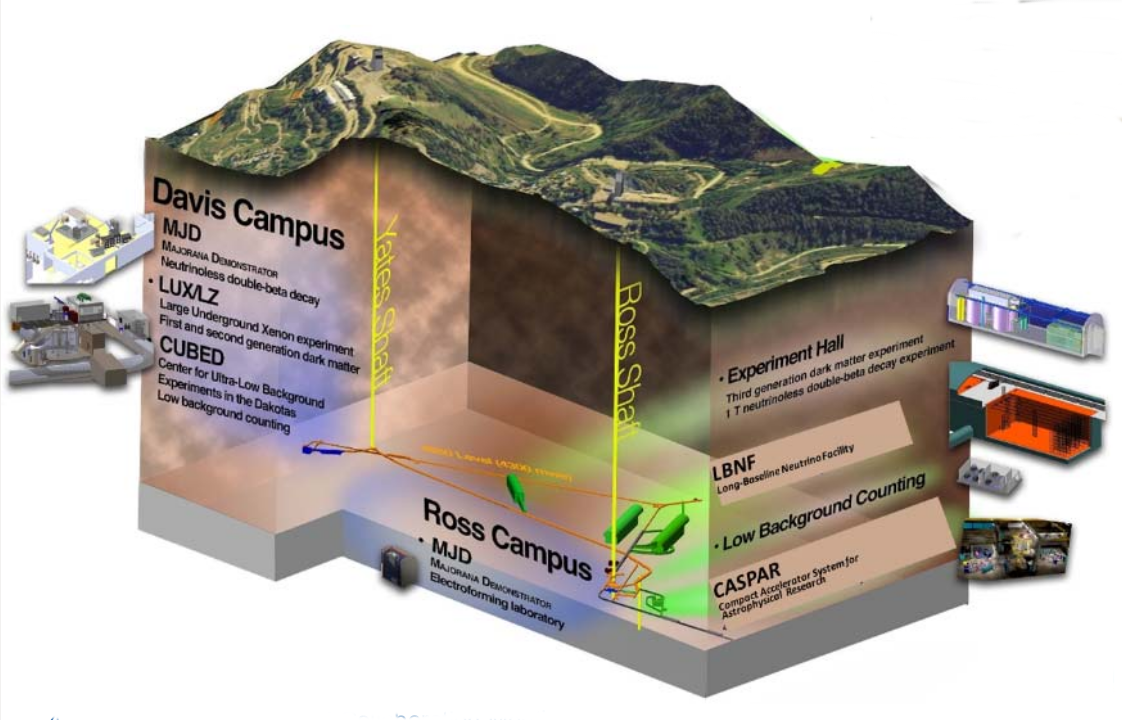
\includegraphics[width=0.95\textwidth, keepaspectratio=true]{figs/farDetector_SanfordUndergroundResearchFacility.png}
\end{figure}

\begin{figure}
\caption{Sanford Underground Research Facility (SURF)}
\label{fig:farDetector_SURF2}
\centering
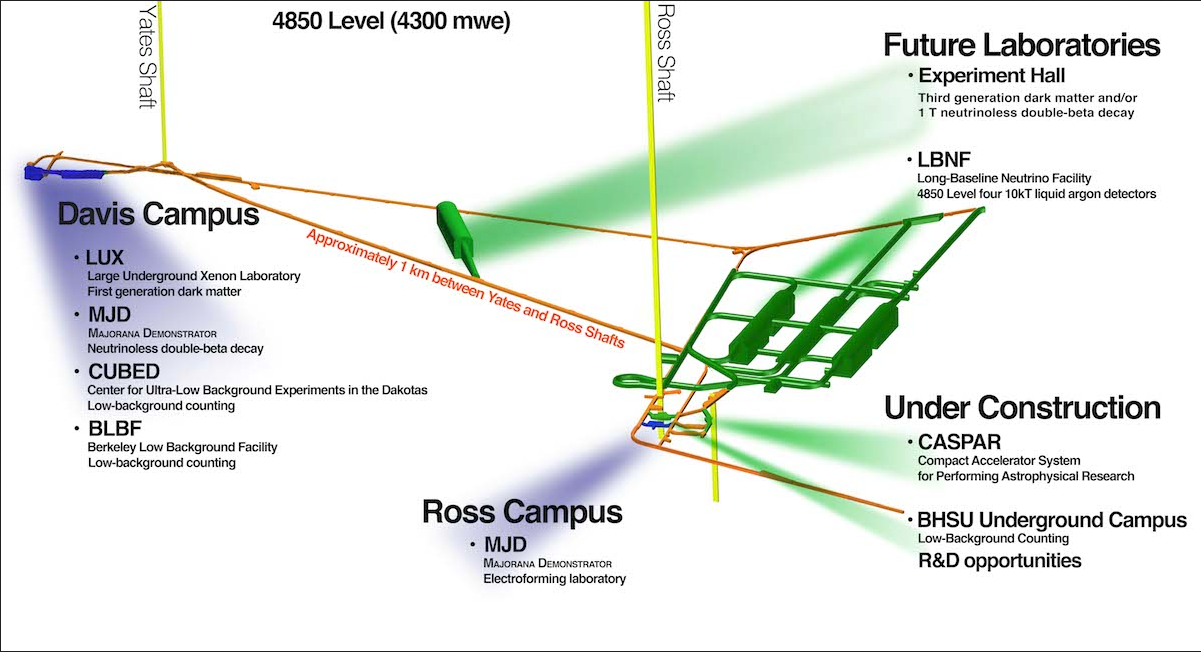
\includegraphics[width=0.95\textwidth, keepaspectratio=true]{figs/farDetector_wholeLab.png}
\end{figure}

\begin{SCfigure}
% side caption
\caption{The scheme of the cross section of the LArTPC for far detector of the DUNE. Source of figure: [REFERENCE]}
\label{fig:farDetector_TPC}
\centering
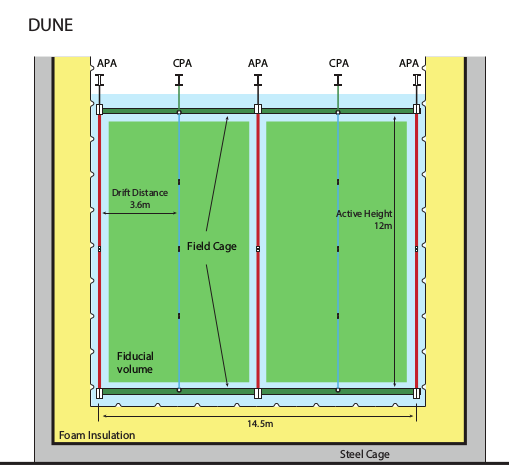
\includegraphics[width=0.50\textwidth, keepaspectratio=true]{figs/farDetector_TPC.png}
\end{SCfigure}

The TPC is particle identification system of the detector. The chamber is merged into the liquid argon at tempetature of 89 K. On the figure \ref{fig:LBNF_TPC} the cathod plane assemblies (CPAs) and the anode plane assemblies (APAs) are shown. The voltages on the APAs and the CPAs are applied in such a way to create unifoem electric field between anode and cathod planes. Chargedparticle traveling though the electron field ionizes argon atoms. Electrons induced in the ionization process drift to the APAs and produce signal on the readout electronic elements.
The important requirements to the TPC include:

\begin{itemize}
  \item be able to perform electron/photon discrimination
  \item wire sag shouldn't affect the position and energy resolutions
  \item discriminate electrons coming from photon conversion from primary electrons
  \item has good performance in measurements of high-energy and low-energy tracks
  \item make sure that materials used wouldn't contaminate high purity argon
\end{itemize}

% [Not sure whether it's good idea to place data aquisition system here, paper should concentrate on physics and major detector schemes]
%The scheme of the data aquisition system is showm on figure \ref{fig:LBNF_DAQ}. The data aquisition is performed in two steps. First, data are triggered by software trigger farm. Then the data which passed trigger requirement are collected.

%\begin{figure}
%\caption{Block Diagram of the Data Aquisition System for the Far Detector of DUNE}
%\label{fig:LBNF_DAQ}
%\centering
%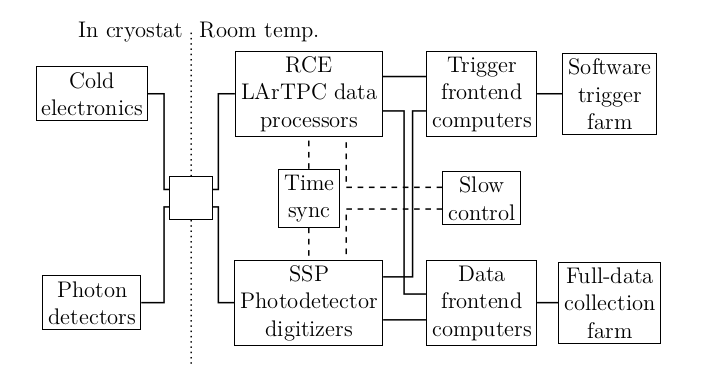
\includegraphics[width=0.70\textwidth, keepaspectratio=true]{figs/LBNF_DAQ.png}
%\\The scheme of the cross section of the LArTPC for far detector of the DUNE compared to LBNE (old experiment).   
%\end{figure}

\subsection{LBNF compared to the other long baseline neutrino oscillation experiments}
The review article\cite{ref_LBN_OscExpReview} describes beams and detectors of long baseline neutrino experiments KEK\cite{ref_KEK}, NuMI\cite{ref_NuMI}, CNGS\cite{ref_CNGS} and J-PARC\cite{ref_JPARC}. The main parameters are summarizet in the table [REFERENCE]

\begin{table}[h]
  \centering
  \begin{center}
  \caption{ Comparison of different long baseline neutrino oscillations experiments}
  \begin{tabular}{|c|c|c|c|c|c|}
              & KEK (K2K) & NuMI & CNGS & T2K & LBNF (DUNE)\\ \hline
     location &   &  &  &  & \\ \hline
     accelerator &   &  &  &  & \\ \hline
     time of operation &   &  &  &  & future \\ \hline 
     beam power  &  5 kW  & 300-350 kW  & 300 kW & 750 kW & \\ \hline 
     energy of protons  & 12 GeV & 120 GeV & 400 GeV & 30 GeV & \\ \hline 
     baseline  & 250 km & 735 km & 730 km & 295 km & 1300 km\\ \hline 
     near detector(s)  &   &  &  &  & \\ \hline 
     far detector(s)  &   &  &  &  & \\ \hline 
 \end{tabular}
  \label{tab:LeptonFlavorNumber}
  \end{center}
\end{table}



